\documentclass{article}
\usepackage{amsmath}
\usepackage{amssymb}
\usepackage{amsthm}
\usepackage{MnSymbol}
\usepackage{xcolor}
\usepackage{parskip}
\usepackage{tikz}
\usetikzlibrary{trees}


\theoremstyle{definition}
\newtheorem{definition}{Definition}
\newtheorem{theorem}{Theorem}


\newcommand{\abs}[1]{\left| #1 \right|}


\title{lecture}
\date{\today}
\begin{document}
\maketitle

\begin{definition}[Clustering]
    given a dataset \(S=\{x_1,x_2,\dots,x_n\}\), find "similar" points
\end{definition}

\(G(V,E,w)\)

\(V\) is verticies, \(E\) is edges

\(w \) is the "weight"

"size of cut" talks about how much weight is removed

examples: clustering time series, K-center, median, mean

given an arbitrary metric space, minimize distance to centers w k (fixed) centers, 



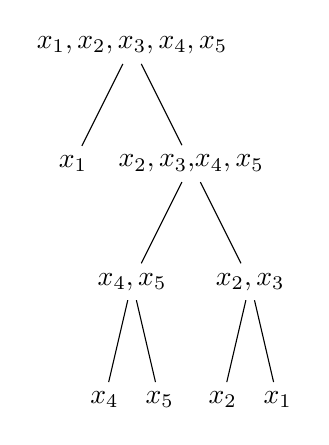
\begin{tikzpicture}[      
    level 1/.style={sibling distance=1.5cm},
    level 2/.style={sibling distance=1.5cm},
    level 3/.style={sibling distance=0.7cm},
    % every node/.style={circle,draw}
]
    \node{\(x_1,x_2,\\x_3,x_4,x_5\)}
    child{node {\(x_1\)} }
    child{
        node {\(x_2,x_3,\)\\\(x_4,x_5\)} 
        child {
            node{\(x_4,x_5\)} child{node{\(x_4\)}}child{node{\(x_5\)}}} 
        child{
            node{\(x_2,x_3\)} child{node{\(x_2\)}}child{node{\(x_1\)}}}};


\end{tikzpicture}


example cost function:

\begin{equation}
    \sum_{i,j\in V}w_{ij}: \frac{\text{\# of data points present when node i,j split}}{n}
\end{equation}




linkage algos: single, average, complete

divisive (top-down), balanced, sparsest


example:
\(G(V,E,w\geq 0)\) \(\abs{V}=n\)



find a binary tree that minimizes cost 
\begin{equation}
    \sum_{ij,\in E} w_{ij}\abs{\text{\# leaves of $T_{ij}$}}
\end{equation}


\(T_{ij}=\) is also called \emph{lowest common ancestor} of \(i,j\)


tree reconstruction problem, use vector reconstruction

\section{Convex Relaxations}
assign a \(\{0,1\}\) variable for each pair of nodes, \(x_{ij}\)

want to represent that we want to look for tree with 0 1 variables, and also represent the objective with 01

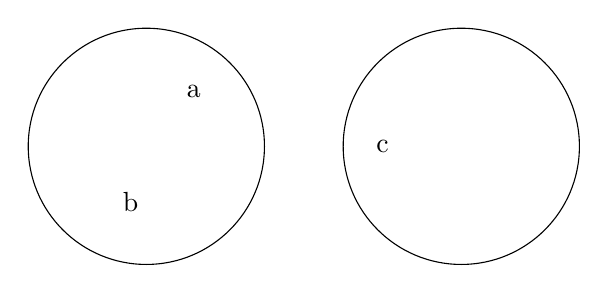
\begin{tikzpicture}
    \draw (0,0) circle [radius=1.5] ;
    \draw (4,0) circle [radius = 1.5];
    \node at (0.6,0.7) {a};
    \node at (-0.2,-0.7) {b};
    \node at (3,0) {c};
\end{tikzpicture}



\(x_{a,b} = 1 \)
\(x_{a,c} = 0 \)

\begin{equation}
    \max_{\text{assigned $\vec x$}}\sum_{ij\in E} w_{ij}x_{ij}
\end{equation}

this system maximizes the "weight cut" in the original cluster finding problem






\end{document}